\documentclass[../notes.tex]{subfiles}
\graphicspath{{\subfix{../images/}}, {\subfix{../}}}

\begin{document}
	
\chapter{Dressed Graphene Model}	

\section{Lattice Structure of Graphene}\label{sec:lattice-structure-of-graphene}

Structure of honeycomb lattice following~\cite{yangStructureGrapheneIts2018}.

Monolayer graphene forms a hexagonal lattice.
%This is formed by two triangular sub lattices.
%So in the unit cell of the hexagonal actually has two atoms.

Primitive lattice vectors of the hexagonal lattice:
\begin{align}
	\vb{a}_1 &= \frac{a}{2} \begin{pmatrix} 1 \\ \sqrt{3} \end{pmatrix} \\
	\vb{a}_2 &= \frac{a}{2} \begin{pmatrix} 1 \\ -\sqrt{3} \end{pmatrix}
\end{align}
with lattice constant \(a \approx \SI{2.46}{\angstrom}\) (distance between unit cells).
Have
\begin{equation}
	a = \sqrt{3} a_0
\end{equation}
with the nearest-neighbour distance \(a_0\).

\begin{figure}[htb]
	\centering
	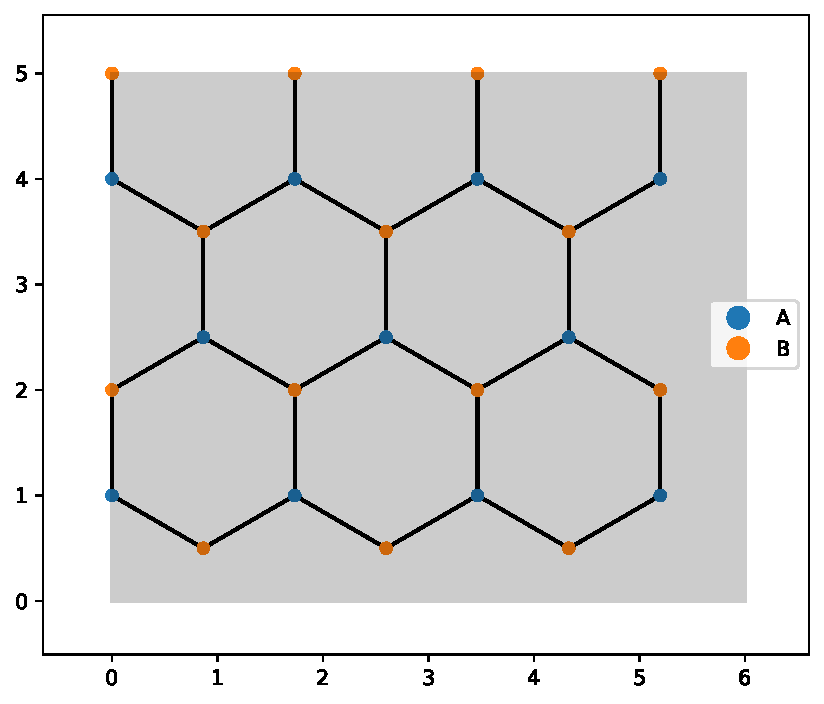
\includegraphics[width=0.7\textwidth]{images/graphene lattice}
	\caption{Graphene lattice structure}
	\label{fig:graphene lattice structure}
\end{figure}

Vectors to the nearest-neighbor \(B_i\) (\(i = 1, 2, 3,\)) atoms from atom \(A\):
\begin{align}
	\vb{\delta}_{AB, 1} = \begin{pmatrix} 0 \\ \frac{a}{\sqrt{3}} \end{pmatrix}, \vb{\delta}_{AB, 2} = \begin{pmatrix} \frac{a}{2} \\ -\frac{a}{2\sqrt{3}} \end{pmatrix}, \vb{\delta}_{AB, 3} = \begin{pmatrix} -\frac{a}{2} \\ -\frac{a}{2\sqrt{3}} \end{pmatrix}
\end{align}

Vectors to the nearest-neighbor \(A_i\) (\(i = 1, 2, 3,\)) atoms from atom \(B\):
\begin{align}
	\vb{\delta}_{BA, 1} = \begin{pmatrix} 0 \\ -\frac{a}{\sqrt{3}} \end{pmatrix}, \vb{\delta}_{BA, 2} = \begin{pmatrix} \frac{a}{2} \\ \frac{a}{2\sqrt{3}} \end{pmatrix}, \vb{\delta}_{BA, 3} = \begin{pmatrix} -\frac{a}{2} \\ \frac{a}{2\sqrt{3}} \end{pmatrix}
\end{align}

The vectors between the Graphene \(\mathrm{A}\) atom and the six neighbours on the same sub lattice can be found by rotating \(\vb{a}_1\) six times by \(\nicefrac{1}{6} * 2\pi = \nicefrac{\pi}{3}\):
\begin{align}
	\vb{\delta}_{AA, 1} &= \vb{a}_1 = \frac{a}{2} \begin{pmatrix} 1 \\ \sqrt{3} \end{pmatrix} = a \begin{pmatrix} \frac{1}{2} \\ \frac{\sqrt{3}}{2} \end{pmatrix} = a \begin{pmatrix} \sin{(\frac{\pi}{6})} \\ \cos{(\frac{\pi}{6})} \end{pmatrix} \\
	\vb{\delta}_{AA, 2} &= a \begin{pmatrix} \sin{(\frac{3\pi}{6})} \\ \cos{(\frac{3\pi}{6})} \end{pmatrix} = a \begin{pmatrix} 1 \\ 0 \end{pmatrix} \\
	\vb{\delta}_{AA, 3} &= a \begin{pmatrix} \sin{(\frac{5\pi}{6})} \\ \cos{(\frac{5\pi}{6})} \end{pmatrix} = a \begin{pmatrix} \frac{1}{2} \\ -\frac{\sqrt{3}}{2} \end{pmatrix} \\
	\vb{\delta}_{AA, 4} &= a \begin{pmatrix} \sin{(\frac{7\pi}{6})} \\ \cos{(\frac{7\pi}{6})} \end{pmatrix} = a \begin{pmatrix} -\frac{1}{2} \\ -\frac{\sqrt{3}}{2} \end{pmatrix} \\
	\vb{\delta}_{AA, 5} &= a \begin{pmatrix} \sin{(\frac{9\pi}{6})} \\ \cos{(\frac{9\pi}{6})} \end{pmatrix} = a \begin{pmatrix} -1 \\ 0 \end{pmatrix} \\
	\vb{\delta}_{AA, 6} &= a \begin{pmatrix} \sin{(\frac{11\pi}{6})} \\ \cos{(\frac{11\pi}{6})} \end{pmatrix} = a \begin{pmatrix} -\frac{1}{2} \\ \frac{\sqrt{3}}{2} \end{pmatrix}
\end{align}

\begin{figure}[htb]
	\centering
	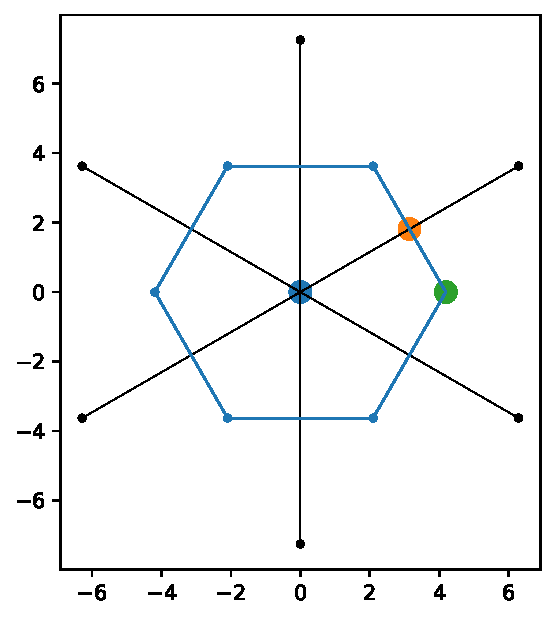
\includegraphics[width=0.5\textwidth]{images/graphene brillouin_zone}
	\caption{Graphene Brillouin Zone}
	\label{fig:graphene Brillouin zone}
\end{figure}

The primitive reciprocal lattice vectors \(\vb{b}_1\), \(\vb{b}_2\) fulfill
\begin{align}
	\vb{a}_1 \cdot \vb{b}_1 &= \vb{a}_2 \cdot \vb{b}_2 = 2\pi \\
	\vb{a}_1 \cdot \vb{b}_2 &= \vb{a}_2 \cdot \vb{b}_1 = 0
	\;,
\end{align}
so we have:
\begin{align}
	\vb{b}_1 &= \frac{2\pi}{a} \begin{pmatrix} 1 \\ \frac{1}{\sqrt{3}} \end{pmatrix} \\
	\vb{b}_2 &= \frac{2\pi}{a} \begin{pmatrix} 1 \\ - \frac{1}{\sqrt{3}} \end{pmatrix}
\end{align}
Points of high symmetry in the Brillouin zone are:
\begin{align}
	\Gamma &= \begin{pmatrix} 0 \\ 0 \end{pmatrix} \\
	\mathrm{M} &= \frac{\pi}{a} \begin{pmatrix} 1 \\ \frac{1}{\sqrt{3}} \end{pmatrix} \\
	\mathrm{K} &= \frac{4\pi}{3 a} \begin{pmatrix} 1 \\ 0 \end{pmatrix}
\end{align}

\section{EG-X Model}\label{sec:eg-x-model}

Graphene lattice and a site X\@.
\begin{figure}[htb]
	\centering
	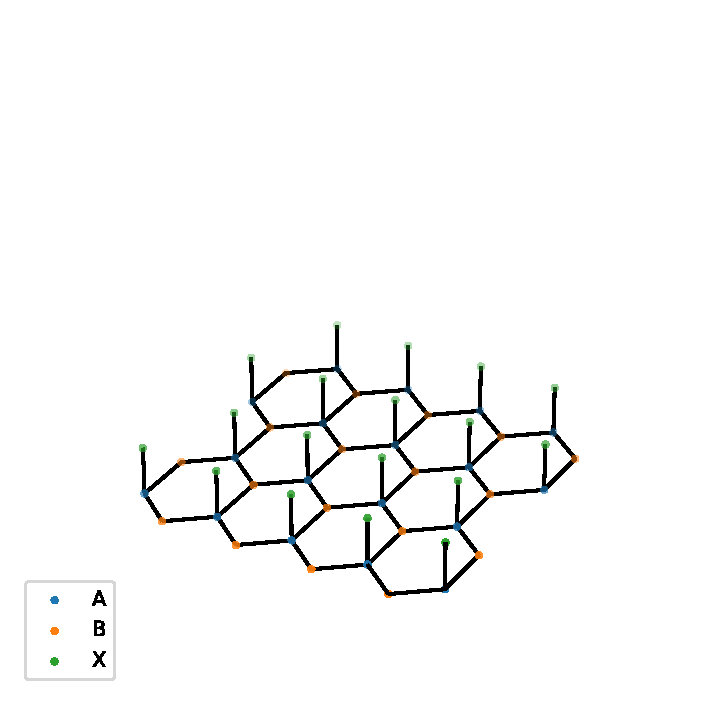
\includegraphics[width=0.5\textwidth]{images/eg-x lattice}
	\caption{EG-X model}
	\label{fig:eg-x model}
\end{figure}
Real-life motivation: layer of graphene on top of a substrate of another material (which provides the additional X atoms).
There is no spin-orbit coupling considered in the model (but when according to Niklas: when mapping to substrates Sn or Pb, it could be necessary (but does not the qualitative result?)).

Without interaction \todo{Spin-orbit coupling, drop second spin index?}:
\begin{align}
	H_0 &= -t_{\mathrm{X}} \sum_{\langle ij \rangle, \sigma \sigma^{\prime}} d_{i, \sigma}^{\dagger} d_{j, \sigma^{\prime}} + \mathrm{h.c.}
	-t_{\mathrm{Gr}} \sum_{\langle ij \rangle, \sigma \sigma^{\prime}} \left(
	c_{i, \sigma}^{(A), \dagger} c_{j, \sigma^{\prime}}^{(B)} +
	c_{j, \sigma^{\prime}}^{(B), \dagger} c_{i, \sigma}^{(A)} + \mathrm{h.c.}
	\right) \\
	&+ V \sum_{i, \sigma \sigma^{\prime}} \left(
	d_{i, \sigma}^{\dagger} c_{i, \sigma^{\prime}}^{(A)} +
	c_{i, \sigma}^{(A), \dagger} d_{i, \sigma^{\prime}}
	\right)
	\label{eq:EG-X model Hamiltonian non-interacting}
\end{align}
with:
\begin{itemize}
	\item \(d\) operators on the X atom
	\item \(c^{(\epsilon)}\) operators on the graphene site (\(\epsilon = A, B\))
	\item \(t_X\) NN hopping for X
	\item \(t_{Gr}\) NN hopping of Gr
	\item \(V\) hybridization between \(\mathrm{X}\) and Graphene \(\mathrm{B}\) sites
\end{itemize}
We can also introduce an onsite Hubbard interaction:
\begin{equation}
	H_{\mathrm{int}} = U_{\mathrm{X}} \sum_{i} d_{i, \uparrow}^{\dagger} d_{i, \downarrow}^{\dagger} d_{i, \downarrow} d_{i, \uparrow}
	+ U_{\mathrm{Gr}} \sum_{i, \epsilon=A, B} c_{i, \uparrow}^{(\epsilon) \dagger} c_{i, \downarrow}^{(\epsilon) \dagger} c_{i, \downarrow}^{\epsilon} c_{i, \uparrow}^{\epsilon}
\end{equation}

\subsection{Review: Hubbard model on the honeycomb lattice}\label{subsec:review:-hubbard-model-on-the-honeycomb-lattice}

\todo{Write review for Hubbard model on the honeycomb lattice}

\subsection{Band structure of the non-interacting EG-X model}\label{subsec:band-structure-of-the-non-interacting-eg-x-model}

To treat eq.~\ref{eq:EG-X model Hamiltonian non-interacting}, we first write out the sums over nearest neighbours \(\langle i, j \rangle\) explicitly, writing \(\vb{\delta}_{\mathrm{X}}, \vb{\delta}_{\epsilon}\) (\(\epsilon = A, B\)) for the connections to the nearest neighbours of the \(\mathrm{X}\) atoms and Graphene \(A, B\) sites.
Doing the calculation for the example of the \(\mathrm{X}\) atoms:
\begin{align}
	&-t_{\mathrm{X}} \sum_{\langle ij \rangle, \sigma \sigma^{\prime}} (d_{i, \sigma}^{\dagger} d_{j, \sigma^{\prime}} + d_{j, \sigma}^{\dagger} d_{i, \sigma^{\prime}}) \\
	&= -\frac{t_X}{2} \sum_{i,\sigma, \sigma^{\prime}} \sum_{\delta_{\mathrm{X}}} d_{i, \sigma}^{\dagger} d_{i + \delta_{\mathrm{X}}, \sigma^{\prime}}
	-\frac{t_X}{2} \sum_{j,\sigma, \sigma^{\prime}} \sum_{\delta_{\mathrm{X}}} d_{j, \sigma}^{\dagger} d_{j + \delta_{\mathrm{X}}, \sigma^{\prime}} \\
	&= -t_X \sum_{i,\sigma, \sigma^{\prime}} \sum_{\delta_{\mathrm{X}}} d_{i, \sigma}^{\dagger} d_{i + \delta_{\mathrm{X}}, \sigma^{\prime}}
	\label{eq:EG-X model X atoms nearest neighbours written out}
\end{align}
(The factor \(\nicefrac{1}{2}\) is to account for double counting when going to the sum over all lattice sites \(i\))

Now we can input the discrete Fourier transform (for both graphene and X operators) into eq.~\ref{eq:EG-X model X atoms nearest neighbours written out}
\begin{align}
	c_{i} &= \frac{1}{\sqrt{N}} \sum_{\vb{k}} e^{\iu \vb{k} \vb{r}_{i}} c_{\vb{k}} \\
	c_{i}^{\dagger} &= \frac{1}{\sqrt{N}} \sum_{\vb{k}} e^{-\iu \vb{k} \vb{r}_{i}} c_{\vb{k}}^{\dagger}
\end{align}
with the completeness relation:
\begin{equation}
	\sum_{i} e^{\iu \vb{k} \vb{r}_{i}} e^{-\iu \vb{k}^{\prime} \vb{r}_{i}} = N \delta_{\vb{k}, \vb{k}^{\prime}}
	\;.
\end{equation}
We get:
\begin{align}
	-t_X \frac{1}{N} \sum_{i,\sigma, \sigma^{\prime}} \sum_{\vb{\delta}_{\mathrm{X}}} d_{i, \sigma}^{\dagger} d_{i + \vb{\delta}_{\mathrm{X}}, \sigma^{\prime}}
	&= -t_X \frac{1}{N} \sum_{i,\sigma, \sigma^{\prime}} \sum_{\vb{\delta}_{\mathrm{X}}} \sum_{\vb{k}, \vb{k}^{\prime}} e^{-\iu \vb{k} \vb{r}_i} d_{\vb{k}, \sigma}^{\dagger} e^{\iu \vb{k}^{\prime} \vb{r}_i} e^{\iu \vb{k}^{\prime} \vb{\delta}_{\mathrm{X}}} d_{\vb{k}^{\prime}, \sigma^{\prime}} \\
	&= -t_X \frac{1}{N} \sum_{\vb{k}, \vb{k^{\prime}}, \sigma, \sigma^{\prime}} \sum_{\vb{\delta}_{\mathrm{X}}} d_{\vb{k}, \sigma}^{\dagger}  e^{\iu \vb{k}^{\prime} \vb{\delta}_{\mathrm{X}}} d_{\vb{k}^{\prime}, \sigma^{\prime}} \sum_{i} e^{-\iu \vb{k} \vb{r}_i} e^{\iu \vb{k}^{\prime} \vb{r}_i} \\
	&= -t_X \frac{1}{N} \sum_{\vb{k}, \vb{k^{\prime}}, \sigma, \sigma^{\prime}} \sum_{\vb{\delta}_{\mathrm{X}}} d_{\vb{k}, \sigma}^{\dagger}  e^{\iu \vb{k}^{\prime} \vb{\delta}_{\mathrm{X}}} d_{\vb{k}^{\prime}, \sigma^{\prime}} N \delta_{\vb{k}, \vb{k}^{\prime}} \\
	&= -t_X \sum_{\vb{k}, \sigma, \sigma^{\prime}}  d_{\vb{k}, \sigma}^{\dagger}d_{\vb{k}, \sigma^{\prime}} \sum_{\vb{\delta}_{\mathrm{X}}} e^{\iu \vb{k} \vb{\delta}_{\mathrm{X}}}
\end{align}
The nearest neighbours for \(\mathrm{X}\) atoms are the vectors \(\vb{\delta}_{AA, i}\) from section~\ref{sec:lattice-structure-of-graphene}.
With that, we can calculate:
\begin{align}
	f_{\mathrm{X}} (\vb{k}) &= -t_X \sum_{\vb{\delta}_{\mathrm{X}}} e^{\iu \vb{k} \vb{\delta}_{\mathrm{X}}} \\
	&= -t_X \left( e^{\iu a (\frac{k_x}{2} + \frac{\sqrt{3} k_y}{2})}
	+ e^{\iu a k_x}
	+ e^{\iu a (\frac{k_x}{2} - \frac{\sqrt{3} k_y}{2})}
	\right. \\
	&+ \left. e^{\iu a (-\frac{k_x}{2} - \frac{\sqrt{3} k_y}{2})}
	+ e^{-\iu a k_x}
	+ e^{\iu a (-\frac{k_x}{2} + \frac{\sqrt{3} k_y}{2})} \right) \\
	&= -t_X \left( 2 \cos{(a k_x)} + 2 e^{\iu a \frac{\sqrt{3} k_y}{2}} \cos{(\frac{a}{2} k_x)} + 2 e^{-\iu a \frac{\sqrt{3} k_y}{2}} \cos{(\frac{a}{2} k_x)} \right) \\
	&= -2t_X \left( \cos{(a k_x)} + 2 \cos{(\frac{a}{2} k_x)} \cos{(\sqrt{3} \frac{ a}{2} k_y)} \right)
\end{align}
We can do the same for the hopping between Graphene sites, for example :
\begin{align}
	-t_{\mathrm{Gr}} \sum_{\langle ij \rangle, \sigma \sigma^{\prime}} c_{i, \sigma}^{(A), \dagger} c_{j, \sigma^{\prime}}^{(B)}
	&= -t_{\mathrm{Gr}} \sum_{i, \sigma \sigma^{\prime}} \sum_{\vb{\delta}_{AB}} c_{i, \sigma}^{(A), \dagger} c_{i + \vb{\delta}_{AB} , \sigma^{\prime}}^{(B)} \\
	&= -t_{\mathrm{Gr}} \sum_{\vb{k}, \sigma, \sigma^{\prime}}  c_{\vb{k}, \sigma}^{(A) \dagger} c_{\vb{k}, \sigma^{\prime}}^{(B)} \sum_{\vb{\delta}_{AB}} e^{\iu \vb{k} \vb{\delta}_{AB}}
\end{align}
We note
\begin{align}
	\sum_{\vb{\delta}_{AB}} e^{\iu \vb{k} \vb{\delta}_{AB}} = \left( \sum_{\vb{\delta}_{BA}} e^{\iu \vb{k} \vb{\delta}_{BA}} \right)^* = \sum_{\vb{\delta}_{BA}} e^{-\iu \vb{k} \vb{\delta}_{BA}}
\end{align}
and calculate
\begin{align}
	f_{Gr} &= -t_{Gr} \sum_{\vb{\delta}_{AB}} e^{\iu \vb{k} \vb{\delta}_{AB}} \\
	&= -t_{Gr} \left(
	e^{\iu \frac{a}{\sqrt{3}} k_y} +
	e^{\iu \frac{a}{2\sqrt{3}} (\sqrt{3} k_x - k_y)} +
	e^{\iu \frac{a}{2\sqrt{3}} (-\sqrt{3} k_x - k_y)} \right) \\
	&= -t_{Gr} \left(
	e^{\iu \frac{a}{\sqrt{3}} k_y} +
	e^{-\iu \frac{a}{2\sqrt{3}} k_y} \left(
	e^{\iu \frac{a}{2} k_x} + e^{-\iu \frac{a}{2} k_x}
	\right) \right) \\
	&= -t_{Gr} \left(
	e^{\iu \frac{a}{\sqrt{3}} k_y} +
	2 e^{-\iu \frac{a}{2\sqrt{3}} k_y}
	\cos{(\frac{a}{2} k_x)} \right)
\end{align}
All together, we get:
\begin{align}
	H_0 &= \sum_{\vb{k}, \sigma, \sigma^{\prime}} \begin{pmatrix} c_{k, \sigma}^{A, \dagger} & c_{k, \sigma}^{B, \dagger} & d_{k, \sigma}^{\dagger} \end{pmatrix}
	\begin{pmatrix}
		0 & f_{Gr} & V \\
		f_{Gr}^* & 0 & 0 \\
		V & 0 & f_{X}
	\end{pmatrix} \begin{pmatrix} c_{k, \sigma}^{A} \\ c_{k, \sigma}^{B} \\ d_{k, \sigma} \end{pmatrix}
	\label{eq:EG-X Hamiltonian non-interacting matrix}
\end{align}
The band structure for the non-interacting EG-X model is easily obtained by diagonalising the matrix in eq.~\ref{eq:EG-X Hamiltonian non-interacting matrix}.
This was done in fig.~\ref{fig:EG-X model non-interacting bands}.

Values used for calculation:
\begin{itemize}
	\item \(a_0 = 1\)
	\item \(t_{\mathrm{Gr}} = 1\)
	\item \(t_{\mathrm{X}} = 0.01\)
\end{itemize}
\(V\) is the control parameter.
(According to Niklas), a range from \(V = 0.1\) to \(V = 2\) can be mapped onto materials in experiment.

\begin{figure}[t]
	\centering
	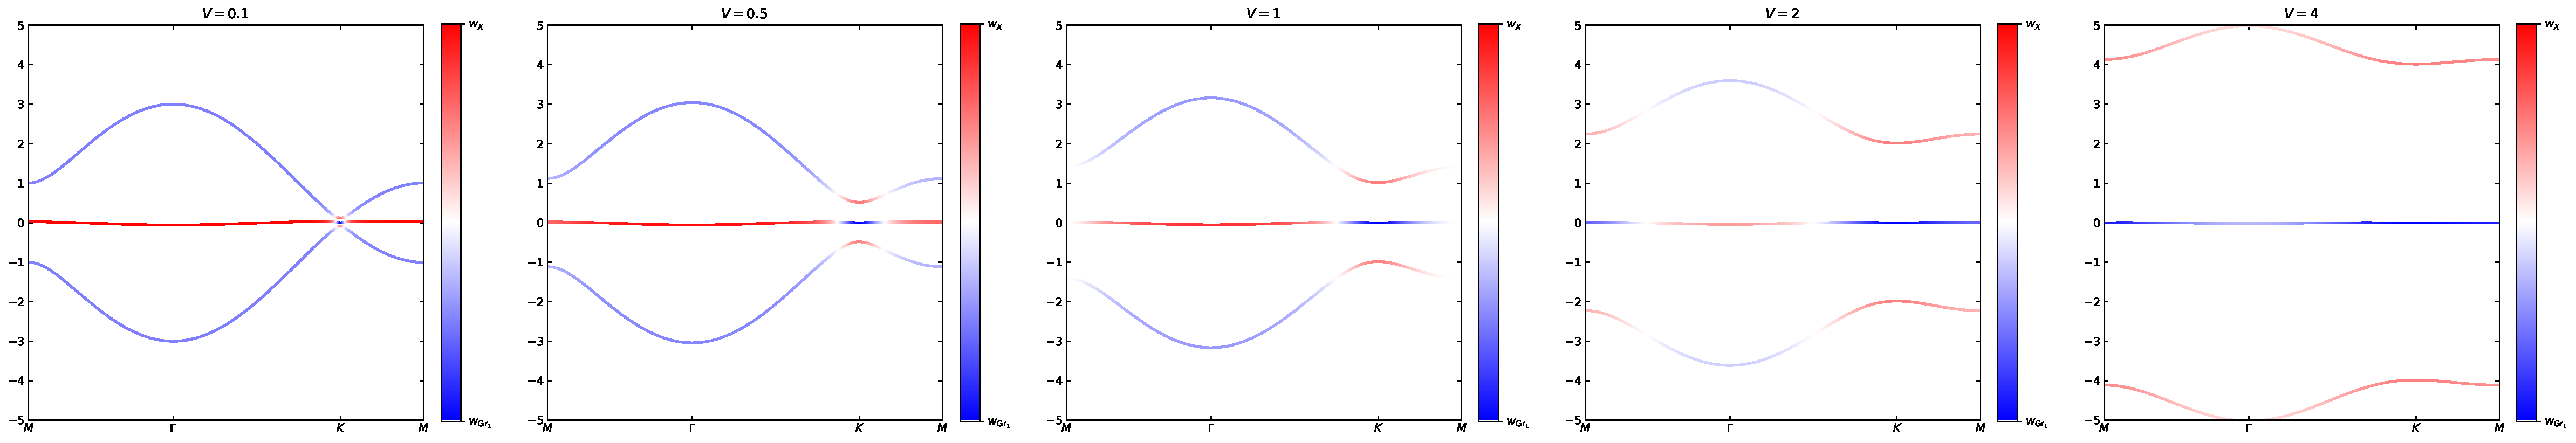
\includegraphics[width=\textwidth]{images/EG_X bands_tGr_1_tX_0.01}
	\caption{Bands of the non-interacting EG-X model. All the bands are spin-degenerate.}
	\label{fig:EG-X model non-interacting bands}
\end{figure}

\section{Multiband BCS?}
	
Define sublattice index
\begin{equation}
	\alpha = 1, 2, 3
\end{equation}
with \(1 \hateq \mathrm{Gr}_1, 2 \hateq \mathrm{Gr}_2, 3 \hateq \mathrm{X}\).
Then we can write the non-interacting term as
\begin{equation}
	H_0 = - \sum_{\langle i, j \rangle, \alpha, \beta, \sigma} \left[\mat{t} \right]_{i\alpha,j\beta} c_{i\alpha}^{\dagger} c_{j\beta}
\end{equation}
with the matrix
\begin{equation}
	\mat{t} = \begin{pmatrix}
		0 & t_{\mathrm{Gr}} & 0 \\
		t_{\mathrm{Gr}} & 0 & -V \delta_{ij} \\
		0 & -V \delta_{ij} & t_{\mathrm{X}} \\
	\end{pmatrix}
\end{equation}

Add chemical potential:
\begin{equation}
	-\mu \sum_{i \alpha \sigma} n_{i \alpha \sigma}
\end{equation}

Also write the interaction part with \(\alpha\) (with changed signs compared to Niklas, to keep in line with papers about the attractive Hubbard model):
\begin{equation}
	H_{int} = - \sum_{i \alpha} U_{\alpha} c_{i\alpha \uparrow}^{\dagger} c_{i\alpha \downarrow}^{\dagger} c_{i\alpha \downarrow} c_{i\alpha \uparrow}
\end{equation}
Fourier transformation:
\begin{equation}
	H_{int} = - \frac{1}{N^2} \sum_{\alpha, \vb{k}_{1, 2, 3, 4}} U_{\alpha} e^{\iu (\vb{k}_1 + \vb{k}_4 - \vb{k}_1 - \vb{k}_3) r_{i \alpha}}  c_{\vb{k}_1 \alpha \uparrow}^{\dagger} c_{\vb{k}_3 \alpha \downarrow}^{\dagger} c_{\vb{k}_2 \alpha \downarrow} c_{\vb{k}_4 \alpha \uparrow}
\end{equation}
Impose zero-momentum pairing: \(\vb{k}_1 + \vb{k}_3 = 0\) and \(\vb{k}_2 + \vb{k}_4 = 0\):
\begin{align}
	H_{int} = - \sum_{\alpha, \vb{k}, \vb{k}^{\prime}} U_{\alpha} c_{\vb{k} \alpha \uparrow}^{\dagger} c_{-\vb{k} \alpha \downarrow}^{\dagger} c_{-\vb{k}^{\prime} \alpha \downarrow} c_{\vb{k}^{\prime} \alpha \uparrow}
\end{align}
Mean-field approximation:
\begin{align}
	H_{int} \approx \sum_{\alpha, \vb{k}} (\Delta_{\alpha} c_{\vb{k} \alpha \uparrow}^{\dagger} c_{-\vb{k} \alpha \downarrow}^{\dagger} + \Delta_{\alpha}^* c_{-\vb{k} \alpha \downarrow} c_{\vb{k} \alpha \uparrow})
\end{align}
with
\begin{align}
	\Delta_{\alpha} &= - U_{\alpha} \sum_{\vb{k}^{\prime}} \braket{c_{-\vb{k}^{\prime} \alpha \downarrow} c_{\vb{k}^{\prime} \alpha \uparrow}} \\
	\Delta_{\alpha}^* &= - U_{\alpha} \sum_{\vb{k}^{\prime}} \braket{c_{\vb{k}^{\prime} \alpha \uparrow}^{\dagger} c_{-\vb{k}^{\prime} \alpha \downarrow}^{\dagger}}
\end{align}
This gives the BCS mean field Hamiltonian:
\begin{align}
	H_{BCS} = \sum_{\vb{k} \alpha \beta \sigma} [H_{0, \sigma} (\vb{k})]_{\alpha \beta} c_{\vb{k} \alpha \sigma}^{\dagger} c_{\vb{k} \beta \sigma}
	-\mu \sum_{\vb{k} \alpha \sigma} n_{\vb{k} \alpha \sigma}
	+ \sum_{\alpha, \vb{k}} (\Delta_{\alpha} c_{\vb{k} \alpha \uparrow}^{\dagger} c_{-\vb{k} \alpha \downarrow}^{\dagger} + \Delta_{\alpha}^* c_{-\vb{k} \alpha \downarrow} c_{\vb{k} \alpha \uparrow})
\end{align}
with Nambu spinor
\begin{equation}
	\Psi_{\vb{k}} =
	\begin{pmatrix}
		c_{1, \vb{k} \uparrow} \\
		c_{2, \vb{k} \uparrow} \\
		c_{3, \vb{k} \uparrow} \\
		c_{1, -\vb{k} \downarrow}^{\dagger} \\
		c_{2, -\vb{k} \downarrow}^{\dagger} \\
		c_{3, -\vb{k} \downarrow}^{\dagger} \\
	\end{pmatrix}
\end{equation}
we have:
\begin{equation}
	H_{MF} = \sum_{\vb{k}} \Psi_{\vb{k}}^{\dagger} \mathcal{H} (\vb{k}) \Psi_{\vb{k}}
\end{equation}
with
\begin{equation}
	\mathcal{H} (\vb{k}) =
	\begin{pmatrix}
		H_{0, \uparrow} (\vb{k}) - \mu & \Delta \\
		\Delta^{\dagger} & - H_{0, \downarrow}^* (-\vb{k}) + \mu
	\end{pmatrix}
\end{equation}
with \(H_{0, \sigma}\) being the F.T. of the kinetic term and \(\Delta = diag(\Delta_1, \Delta_2, \Delta_3)\).


\subsection{BdG Hamiltonian in band basis}

Use transformation
\begin{equation}
	c_{\vb{k} \alpha \sigma}^{\dagger} = \sum_{n} [\mat{G}]_{\alpha n}^* d_{n \vb{k} \sigma}^{\dagger}
\end{equation}
where the columns are made up of the eigenvectors of \(\mat{H}_{0, \sigma}\) for a given \(\vb{k}\):
\begin{equation}
	\mat{G} = 
	\begin{pmatrix}
		\vb{G}_1 & \vb{G}_2 & \vb{G}_3
	\end{pmatrix}
\end{equation}

with that:
\begin{equation}
	\mat{G}^{\dagger}_{\sigma} (\vb{k}) \mat{H}_{0, \sigma} (\vb{k}) \mat{G}_{\sigma} (\vb{k}) =
	\begin{pmatrix}
		\epsilon_1 & 0 & 0 \\
		0 & \epsilon_2 & 0 \\
		0 & 0 & \epsilon_3
	\end{pmatrix}
\end{equation}
So the kinetic part of the BdG Hamiltonian becomes:
\begin{align}
	&\sum_{\vb{k} \alpha \beta \sigma} [H_{0, \sigma} (\vb{k})]_{\alpha \beta}
	\sum_{n} [\mat{G} (\vb{k})]_{\alpha n}^* d_{n \vb{k} \sigma}^{\dagger}
	\sum_{m} [\mat{G} (\vb{k})]_{\beta m} d_{m \vb{k} \sigma}
	-\mu \sum_{\vb{k} \alpha \sigma} n_{n \vb{k} \sigma} \\
	&= \sum_{m n \vb{k} \sigma} d_{n \vb{k} \sigma}^{\dagger} d_{m \vb{k} \sigma}
	\sum_{\alpha \beta} [\mat{G} (\vb{k})]_{\alpha n}^* [H_{0, \sigma} (\vb{k})]_{\alpha \beta} [\mat{G} (\vb{k})]_{\beta m}
	-\mu \sum_{\vb{k} \alpha \sigma} n_{n \vb{k} \sigma} \\
	&= \sum_{m n \vb{k} \sigma} d_{n \vb{k} \sigma}^{\dagger} d_{m \vb{k} \sigma} \epsilon_{n} \delta_{n m}
	-\mu \sum_{\vb{k} \alpha \sigma} n_{n \vb{k} \sigma} \\
	&= \sum_{n \vb{k} \sigma} \epsilon_{n} d_{n \vb{k} \sigma}^{\dagger} d_{n \vb{k} \sigma}
	-\mu \sum_{\vb{k} \alpha \sigma} n_{n \vb{k} \sigma} \\
	&\eqqcolon \sum_{n \vb{k} \sigma} \xi_{\vb{k}} d_{n \vb{k} \sigma}^{\dagger} d_{n \vb{k} \sigma}
\end{align}
with \(\xi_{\vb{k}} \coloneqq \epsilon_{\vb{k}} - \mu\).
The pairing terms become:
\begin{align}
	\sum_{\vb{k} \alpha} \Delta_{\alpha} c_{\vb{k} \alpha \uparrow}^{\dagger} c_{-\vb{k} \alpha \downarrow}^{\dagger}
	&= \sum_{\vb{k} \alpha} \Delta_{\alpha} \sum_n [\mat{G}_{\uparrow} (\vb{k})]_{\alpha n}^* d_{n \vb{k} \uparrow}^{\dagger} \sum_m [\mat{G}_{\downarrow} (-\vb{k})]_{\beta m}^* d_{m -\vb{k} \downarrow}^{\dagger} \\
	&=
\end{align}

So that:
\begin{equation}
	\mathcal{H} (\vb{k}) =
	\begin{pmatrix}
		\epsilon_{\vb{k}} - \mu & G^{\dagger} \Delta G\\
		G^{\dagger} \Delta^{\dagger} G & -\epsilon_{\vb{k}} + \mu
	\end{pmatrix}
\end{equation}
with
\begin{equation}
	\epsilon_{\vb{k}} =
	\begin{pmatrix}
		\epsilon_1 (\vb{k}) & 0 & 0 \\
		0 & \epsilon_2 (\vb{k}) & 0 \\
		0 & 0 & \epsilon_3 (\vb{k}) \\
	\end{pmatrix}
\end{equation}

Concrete example for transformation of gaps from orbital to band basis at \(\mathrm{K} = \frac{4\pi}{3 a} \begin{pmatrix} 1 \\ 0 \end{pmatrix}\).
There, the non-interacting part becomes simply:
\begin{align}
	\mathcal{H}_0 &=
	\begin{pmatrix}
		0 & 0 & V \\
		0 & 0 & 0 \\
		V & 0 & 3 t_X
	\end{pmatrix}
\end{align}
The eigenvalue problem can be solved e.g.~via sympy:
\begin{equation}
	G =
	\begin{pmatrix}
		\frac{- 3 t_{X} - \sqrt{4 V^{2} + 9 t_{X}^{2}}}{\sqrt{4 V^{2} + \left(3 t_{X} + \sqrt{4 V^{2} + 9 t_{X}^{2}}\right)^{2}}} & 0 & \frac{- 3 t_{X} + \sqrt{4 V^{2} + 9 t_{X}^{2}}}{\sqrt{4 V^{2} + \left(3 t_{X} - \sqrt{4 V^{2} + 9 t_{X}^{2}}\right)^{2}}} \\
		0 & 1 & 0 \\
		\frac{2 V}{\sqrt{4 V^{2} + \left(3 t_{X} + \sqrt{4 V^{2} + 9 t_{X}^{2}}\right)^{2}}} & 0 & \frac{2 V}{\sqrt{4 V^{2} + \left(3 t_{X} - \sqrt{4 V^{2} + 9 t_{X}^{2}}\right)^{2}}}
	\end{pmatrix}
\end{equation}
So for \(V \to 0\):
\begin{equation}
	G =
	\begin{pmatrix}
		-1 & 0 & 0 \\
		0 & 1 & 0 \\
		0 & 0 & 1
	\end{pmatrix}
\end{equation}
but for \(V > 0\), there are off-diagonal elements, e.g.~\(V = 0.1\):
\begin{equation}
	G =
	\begin{pmatrix}
		-0.7578 & 0 & 0.6526 \\
		0 & 1 & 0 \\
		0.6526 & 0 & 0.7578
	\end{pmatrix}
\end{equation}
So the transformation of the gap from orbital to band space reads:
\begin{equation}
	G^{\dagger} \Delta G =
	\begin{pmatrix}
		\frac{3 \Delta_{1} t_{X} - 3 \Delta_{3} t_{X} + \left(\Delta_{1} + \Delta_{3}\right) \sqrt{4 V^{2} + 9 t_{X}^{2}}}{2 \sqrt{4 V^{2} + 9 t_{X}^{2}}} & 0 & \frac{V \left(- \Delta_{1} + \Delta_{3}\right)}{\sqrt{4 V^{2} + 9 t_{X}^{2}}} \\
		0 & \Delta_{2} & 0 \\
		\frac{V \left(- \Delta_{1} + \Delta_{3}\right)}{\sqrt{4 V^{2} + 9 t_{X}^{2}}} & 0 & \frac{- 3 \Delta_{1} t_{X} + 3 \Delta_{3} t_{X} + \left(\Delta_{1} + \Delta_{3}\right) \sqrt{4 V^{2} + 9 t_{X}^{2}}}{2 \sqrt{4 V^{2} + 9 t_{X}^{2}}}
	\end{pmatrix}
\end{equation}
So in particular there is no interband pairing for \(V \to 0\):
\begin{equation}
	G^{\dagger} \Delta G =
	\begin{pmatrix}
		\Delta_1 & 0 & 0 \\
		0 & \Delta_{2} & 0 \\
		0 & 0 & \Delta_3
	\end{pmatrix}
\end{equation}
But for \(V > 0\), there is interband pairing (e.g. \(V = 0.1\)):
\begin{equation}
	G^{\dagger} \Delta G =
	\begin{pmatrix}
		0.5742 \Delta_{1} + 0.4258 \Delta_{3} & 0 & - 0.4945 \Delta_{1} + 0.4945 \Delta_{3} \\
		0 & \Delta_{2} & 0 \\
		- 0.4945 \Delta_{1} + 0.4945 \Delta_{3} & 0 & 0.4258 \Delta_{1} + 0.5742 \Delta_{3}
	\end{pmatrix}
\end{equation}

\subsection{Grand potential}

See \cite{peottaSuperfluidityTopologicallyNontrivial2015}, especially supplementary material, notes 1 and 3.

Mean-Field Hamiltonian (with the last two terms due to exchange of anticommuting fermion operators and the term quadratic in the expectation value from the mean-field decoupling respectively):
\begin{equation}
	H_{MF} = \sum_{\vb{k}} \Psi_{\vb{k}}^{\dagger} \mathcal{H} (\vb{k}) \Psi_{\vb{k}} + \sum_{\vb{k}} \Tr(H^{\downarrow}_{\vb{k}}) + \sum_{\vb{k} \alpha} \frac{\vert \Delta_{\alpha} \vert^2}{U}
\end{equation}
The second term is the trace of the non-interacting Hamiltonian.

Thermodynamic grand potential (which at zero temperature is equivalent to the mean-field energy):
\begin{align}
	\Omega (T, \Delta) &= -\frac{1}{\beta} \ln{Z_{\Omega}} = -\frac{1}{\beta} \ln{\Tr(e^{-\beta H_{MF}})} \\
	&= \sum_{\vb{k}} \Tr(H^{\downarrow}_{\vb{k}}) + \sum_{\vb{k} \alpha} \frac{\vert \Delta_{\alpha} \vert^2}{U} - \frac{1}{\beta} \ln{\Tr(e^{-\beta \Psi_{\vb{k}}^{\dagger} \mathcal{H} (\vb{k}) \Psi_{\vb{k}}})}
\end{align}
Zero temperature limit:
\begin{align}
	\Omega (\Delta) &= \sum_{\vb{k}} \Tr(H^{\downarrow}_{\vb{k}}) + \sum_{\vb{k} \alpha} \frac{\vert \Delta_{\alpha} \vert^2}{U} - \frac{1}{2} \sum_{\vb{k}} \Tr([\vert \mathcal{H}_{\vb{k}} \vert])
\end{align}
where a function of a matrix \(H\) (such as taking the absolute value of the BdG Hamiltonian \(\mathcal{H}_{\vb{k}}\)) is defined for the diagonal matrix of eigenvalues \(D\) and the unitary matrix \(U\) that diagonalizes \(H\):
\begin{equation}
	f(H) = U f(D) U^{\dagger}
\end{equation}
The route to finding the value of the order parameter for a fixed interaction \(U\) is minimizing the grand potential with respect to \(\Delta\).




\end{document}
